%
% $RCSfile: misleading_tiers.tex,v $
%
% Copyright (c) 2005-2006. Christian Heller. All rights reserved.
%
% Permission is granted to copy, distribute and/or modify this document
% under the terms of the GNU Free Documentation License, Version 1.1 or
% any later version published by the Free Software Foundation; with no
% Invariant Sections, with no Front-Cover Texts and with no Back-Cover
% Texts. A copy of the license is included in the section entitled
% "GNU Free Documentation License".
%
% http://www.cybop.net
% - Cybernetics Oriented Programming -
%
% http://www.resmedicinae.org
% - Information in Medicine -
%
% Version: $Revision: 1.1 $ $Date: 2006-01-03 08:21:45 $ $Author: christian $
% Authors: Christian Heller <christian.heller@tuxtax.de>
%

\subsection{Misleading Tiers}
\label{misleading_tiers_heading}

When distinguishing human- and technical systems, the kinds of
\emph{Communication} are:

\begin{itemize}
    \item[-] Human $\leftrightarrow$ Human
    \item[-] Human $\leftrightarrow$ Computer
    \item[-] Computer $\leftrightarrow$ Computer
\end{itemize}

Each of these relies on different techniques, transport mechanisms, languages
(protocols) and so on. But the general principle after which communication
works, is always the same -- no matter whether technical \emph{Computer}
systems or their biological prototype, the \emph{Human Being}, are considered:
Information is \emph{received}, \emph{stored}, \emph{processed} and \emph{sent}.
Despite these common characteristics, today's \emph{Information Technology}
(IT) environments \cite{hellerkunze} treat communication between a computer
system and a human being differently than that \emph{among} computer systems.

\begin{figure}[ht]
    \begin{center}
        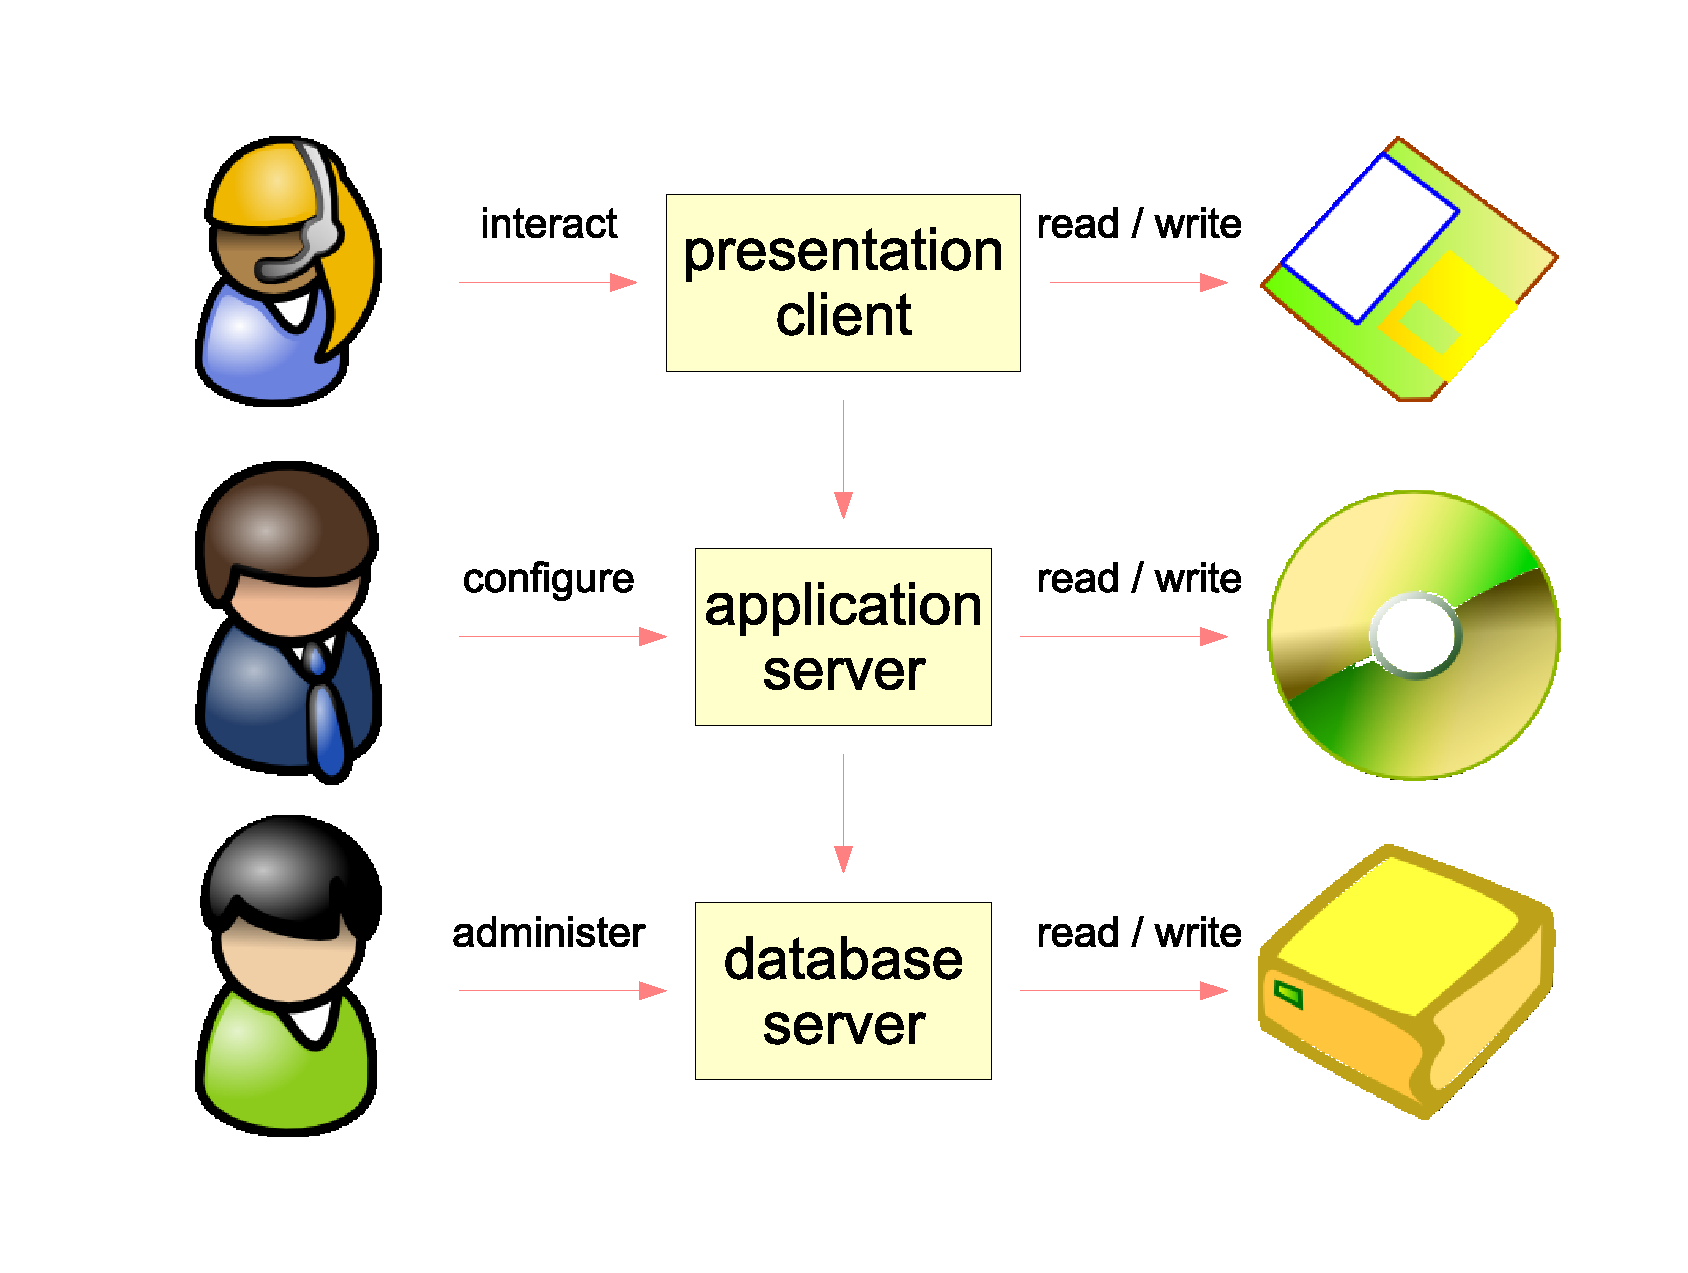
\includegraphics[scale=0.2]{vector/universal.eps}
        \caption{Universal Communication}
        \label{universal_figure}
    \end{center}
\end{figure}

Figure \ref{universal_figure} shows a three-tier environment: tier 1 represents
the \emph{Presentation Layer}; tier 2 stands for the \emph{Application Layer};
tier 3 is the \emph{Database (DB) Layer}. Typical synonyms are, in this order:
\emph{Frontend}, \emph{Business Logic} and \emph{Backend}. The tiers (layers)
serve two needs: connect different locations and share work load (\emph{Scaling}).
However, the split into tiers of that kind raises two illusions:

\begin{enumerate}
    \item \emph{Users only interact with clients}
    \item \emph{Persistent data are stored in DB only}
\end{enumerate}

Many IT architectures, or at least their illustrations, neglect the fact that
in reality \emph{all} systems need a \emph{User Interface} (UI), for at least
being administered by humans, and \emph{almost} all systems, even
\emph{Database Management Systems} (DBMS) themselves, store some of their
persistent data outside a database, for example locally available configuration
information. This is not necessarily a problem for the IT environment as such,
but it is for the internal architecture of software systems. Special solutions
have to deal with frontend (UI framework), business logic (domain patterns) and
backend (data mapping), and often additional mechanisms for local and remote
communication. The serious differences in these design solutions are one root
of well-known problems like multi- directional inter-dependencies between system
parts, that make software difficult to develop and hard to maintain.

One aim of the work described in this article was to investigate possibilities
for a \emph{unification} of communication paradigms, that is high-level design
paradigms rather than low-level protocols, in order to architect software in a
way that allows the computer system it runs on to communicate \emph{universally}.
